%% ============================================================
%%  SECCIÓN 6 — Procedimiento Experimental
%% ============================================================

\section{Procedimiento Experimental}
\label{sec:procedimiento}

\begin{figure}[H]
    \centering
    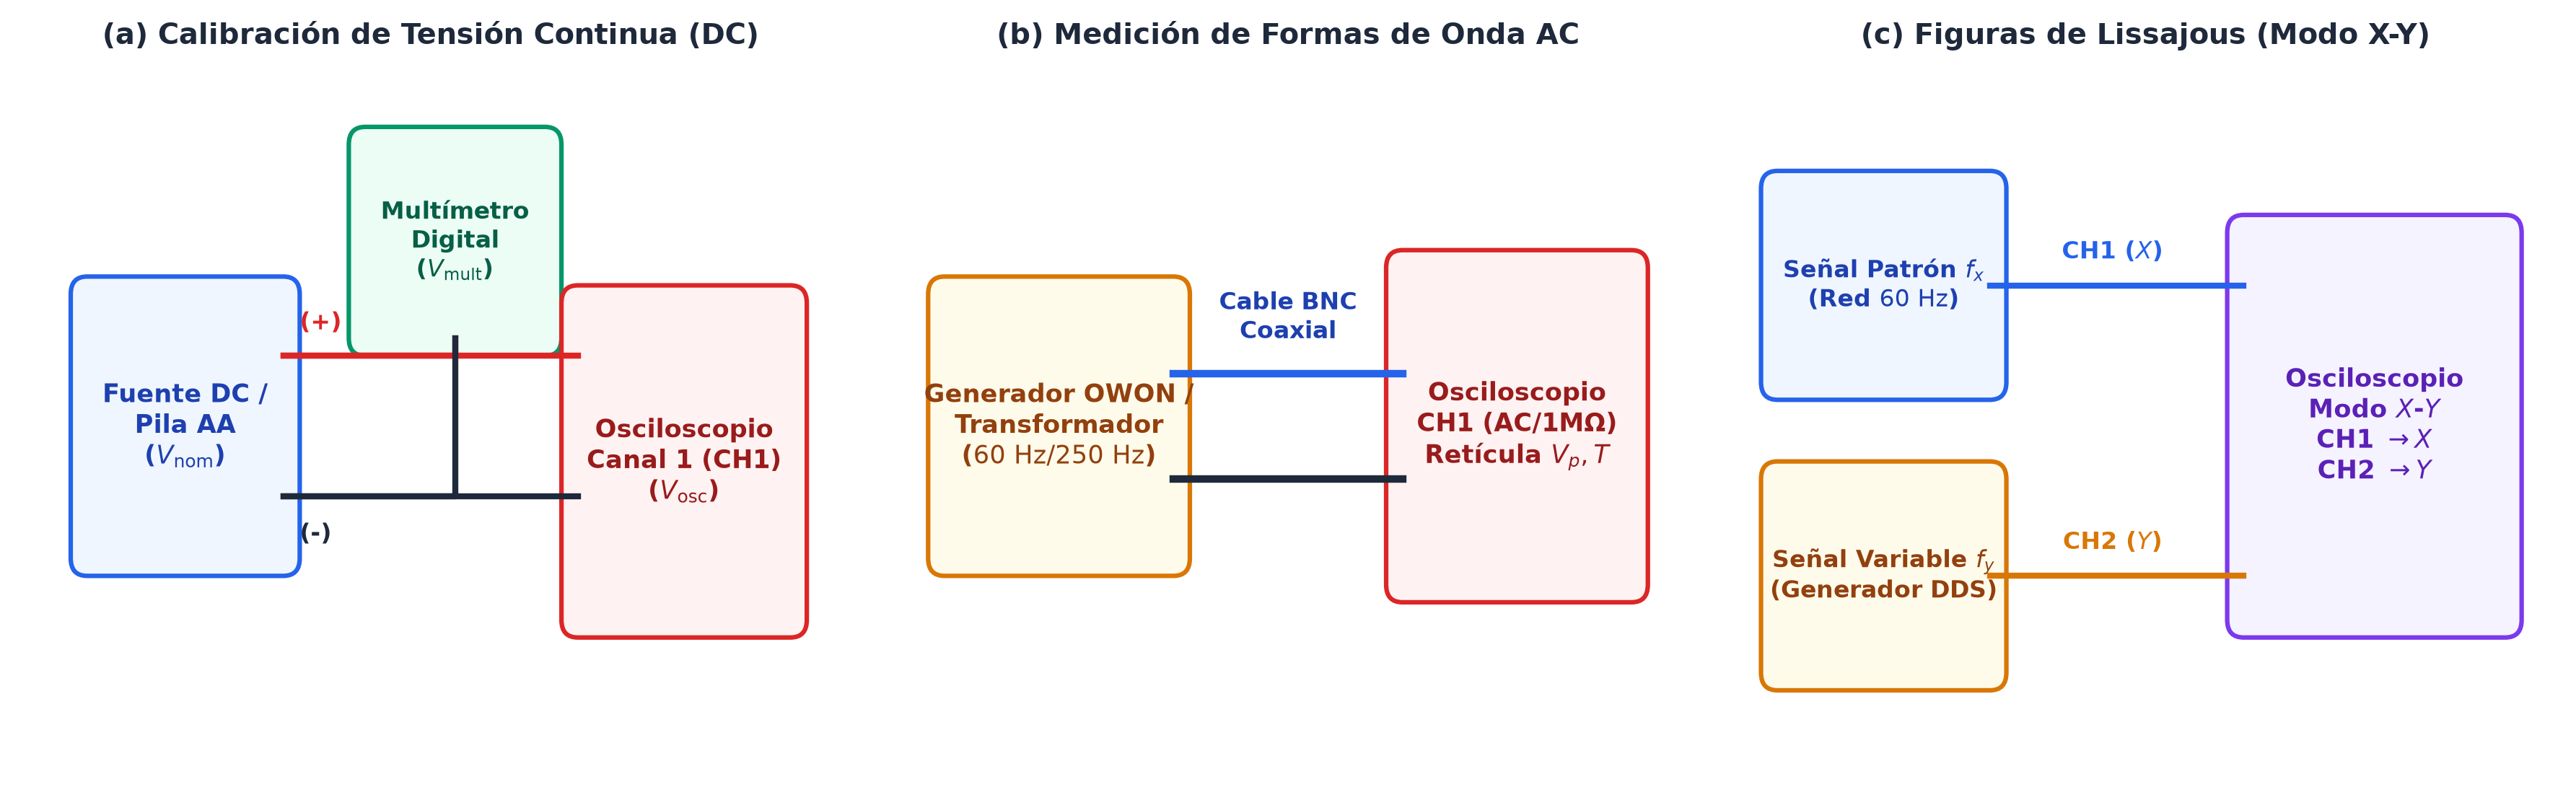
\includegraphics[width=0.95\linewidth]{fig_circuitos_montaje}
    \caption{Esquemas de conexión de los circuitos experimentales empleados en el laboratorio: (a) Calibración de tensión continua en paralelo con multímetro patrón; (b) Medición y sincronización de formas de onda alternas periódicas; (c) Conexión bidimensional en modo $X$-$Y$ para la generación de figuras de Lissajous.}
    \label{fig:circuitos_montaje}
\end{figure}

El desarrollo experimental se estructuró en cinco fases cronológicas consecutivas siguiendo el protocolo de la guía de laboratorio, implementando los esquemas circuitales mostrados en la Figura~\ref{fig:circuitos_montaje}:

\subsection{Parte A: Identificación de Controles y Calibración Inicial}
\begin{enumerate}
    \item Se encendió el osciloscopio digital mediante el interruptor principal y se verificó el ciclo de autocalibración y alineación interna.
    \item Sin conectar potenciales externos a las entradas BNC de los canales $\text{CH1}$ y $\text{CH2}$, se seleccionó el acoplamiento $\text{GND}$ en ambos canales para definir y centrar la línea de referencia horizontal en la retícula central ($y = 0$).
    \item Se ajustó la escala vertical inicial de ambos canales en \qty{1}{\volt\per\division} y la base de tiempo en \qty{1}{\milli\second\per\division}.
\end{enumerate}

\subsection{Parte B: Medición de Voltajes Constantes DC}
\begin{enumerate}
    \setcounter{enumi}{3}
    \item Se configuró el acoplamiento en $\text{DC}$ en el canal $\text{CH1}$.
    \item Se conectó la pila de \qty{1,5}{\volt} al conector BNC de $\text{CH1}$ mediante un cable coaxial. Se varió la perilla de sensibilidad vertical pasando por las escalas de \qty{5}{\volt\per\division}, \qty{2}{\volt\per\division}, \qty{1}{\volt\per\division}, \qty{0,5}{\volt\per\division} y \qty{0,2}{\volt\per\division}, registrando el número de divisiones verticales de deflexión $N_{\text{div}}$ ("al ojo", con apreciación de $0{,}1\,\text{div}$) y determinando la escala óptima.
    \item Se midió simultáneamente la diferencia de potencial de la pila con el multímetro digital patrón.
    \item Se repitió el procedimiento con las distintas salidas fijas de la fuente de alimentación continua (\qty{2,5}{\volt}, \qty{4,5}{\volt}, \qty{7,5}{\volt} y \qty{10,5}{\volt}), registrando las deflexiones y anotando los casos de fuera de escala por saturación vertical.
\end{enumerate}

\subsection{Parte C: Medición de Tensión Alterna AC (Transformador 220 V / 6 V — 60 Hz)}
\begin{enumerate}
    \setcounter{enumi}{7}
    \item Se conectó el devanado secundario del transformador de \qty{6}{\volt} a la entrada $\text{CH1}$ con acoplamiento $\text{AC}$.
    \item Se ajustó la sensibilidad vertical a \qty{5}{\volt\per\division} y \qty{2}{\volt\per\division} para visualizar la forma de onda sinusoidal completa sin distorsión.
    \item Se modificó la base de tiempo horizontal a \qty{5}{\milli\second\per\division}, \qty{2}{\milli\second\per\division} y \qty{1}{\milli\second\per\division}, midiendo el número de divisiones horizontales $N_x$ correspondientes a un ciclo completo (o medio ciclo).
    \item Se activó la función de medición automática (\textit{Quick View}) para registrar el valor numérico medido por el frecuencímetro y voltímetro interno del osciloscopio.
    \item Se midió la tensión eficaz del secundario mediante el multímetro digital True-RMS para contrastar el valor pico teórico ($V_p = \sqrt{2} V_{\text{rms}}$).
\end{enumerate}

\subsection{Parte D: Caracterización de Señales con Generador de Funciones}
\begin{enumerate}
    \setcounter{enumi}{12}
    \item Se conectó la salida del generador OWON AG 051F al canal $\text{CH2}$ del osciloscopio.
    \item Se fijó una frecuencia nominal de \qty{250}{\hertz} y una amplitud de $V_p = \qty{4,80}{\volt}$ ($V_{pp} = \qty{9,60}{\volt}$).
    \item Se seleccionaron sucesivamente tres formas de onda: \textbf{senoidal}, \textbf{triangular} y \textbf{cuadrada}. Para cada una se registró la amplitud pico en \qty{2}{\volt\per\division}, el período en divisiones horizontales ($N_x$) y la tensión eficaz registrada por el multímetro digital.
\end{enumerate}

\subsection{Parte E: Modo Graficador X-Y y Figuras de Lissajous}
\begin{enumerate}
    \setcounter{enumi}{16}
    \item Se habilitó el modo $X$-$Y$ en el menú del osciloscopio, inyectando la señal de \qty{60}{\hertz} del transformador en $\text{CH1}$ (eje $X$) y la señal del generador en $\text{CH2}$ (eje $Y$).
    \item Se ajustó la frecuencia del generador a \qty{60}{\hertz} (relación $1:1$), observando la elipse resultante. Se activó la función de inversión del canal 2 ($\text{CH2 INVERT}$) para registrar el cambio en la orientación espacial de la figura.
    \item Se varió la frecuencia del generador a \qty{120}{\hertz} (relación $1:2$), \qty{180}{\hertz} (relación $1:3$) y \qty{240}{\hertz} (relación $1:4$), registrando la geometría y número de bucles cerrados.
    \item Finalmente, se aplicaron señales continuas constantes (\qty{1,5}{\volt} en $\text{CH1}$ y \qty{3,0}{\volt} en $\text{CH2}$ en modo DC), observando la proyección de un punto estático y su traslación tras invertir el canal 2.
\end{enumerate}